\documentclass[red]{tutorial}
\usepackage[no-math]{fontspec}
\usepackage{xpatch}
	\renewcommand{\ttdefault}{ul9}
	\xpatchcmd{\ttfamily}{\selectfont}{\fontencoding{T1}\selectfont}{}{}
	\DeclareTextCommand{\nobreakspace}{T1}{\leavevmode\nobreak\ }
\usepackage{polyglossia} % English please
	\setdefaultlanguage[variant=us]{english}
%\usepackage[charter,cal=cmcal]{mathdesign} %different font
%\usepackage{avant}
\usepackage{microtype} % Less badboxes


\usepackage[charter,cal=cmcal]{mathdesign} %different font
%\usepackage{euler}
 
\usepackage{blindtext}
\usepackage{calc, ifthen, xparse, xspace}
\usepackage{makeidx}
\usepackage[hidelinks, urlcolor=blue]{hyperref}   % Internal hyperlinks
\usepackage{mathtools} % replaces amsmath
\usepackage{bbm} %lower case blackboard font
\usepackage{amsthm, bm}
\usepackage{thmtools} % be able to repeat a theorem
\usepackage{thm-restate}
\usepackage{graphicx}
\usepackage{xcolor}
\usepackage{multicol}
\usepackage{fnpct} % fancy footnote spacing
\usepackage{tikz}
\usetikzlibrary{arrows.meta}

\usepackage{pgfplots}
\pgfplotsset{compat=1.18}
%\pgfkeys{/pgf/fpu}

 
\newcommand{\xh}{{{\mathbf e}_1}}
\newcommand{\yh}{{{\mathbf e}_2}}
\newcommand{\zh}{{{\mathbf e}_3}}
\newcommand{\R}{\mathbb{R}}
\newcommand{\Z}{\mathbb{Z}}
\newcommand{\N}{\mathbb{N}}
\newcommand{\Proj}{\mathrm{proj}}
\newcommand{\Perp}{\mathrm{perp}}
\renewcommand{\span}{\mathrm{span}\,}
\newcommand{\Span}{\mathrm{span}\,}
\newcommand{\Img}{\mathrm{img}\,}
\newcommand{\Null}{\mathrm{null}\,}
\newcommand{\Range}{\mathrm{range}\,}
\newcommand{\rref}{\mathrm{rref}}
\newcommand{\Rank}{\mathrm{rank}}
\newcommand{\nnul}{\mathrm{nullity}}
\newcommand{\mat}[1]{\begin{bmatrix}#1\end{bmatrix}}
\renewcommand{\d}{\mathrm{d}}


\theoremstyle{definition}
\newtheorem{example}{Example}[section]
\newtheorem{defn}{Definition}[section]

%\theoremstyle{theorem}
\newtheorem{thm}{Theorem}[section]

\pgfkeys{/tutorial,
	name={Tutorial 2},
	author={Jason Siefken \& Bernardo Galv\~ao-Sousa},
	course={MAT 244},
	date={},
	term={},
	title={The Phase Plane}
	}

\begin{document}
	\begin{tutorial}
		%
% Analyze new Phase Portraits
% 1. Give two component graphs of a "solution" and ask them to graph in phase space
% 2. Give a figure 8 in phase space and ask them to draw component graphs so that one loop is traced twice as fast as the other loop
% 3. (a) Can you always go from component graphs to a graph in phase space? What about from a graph in phase space to component graphs? Explain.
% (b) List at least one benefit of (i) component graphs and (ii) graphs in phase space
% 4. Give them the graph from: https://www.desmos.com/calculator/o3xjzddojw
% 
% ask them to identify: (a) where are the equilibria? (b) Classify their
% nature as stable/unstable/etc. How do you know? (c) introduce basins of
% attraction ... (d) Divide the phase space into regions where solutions
% exhibit different natures: where solutions are bounded forwards in time,
% bounded backwards in time, periodic, and unbounded. (e) in which regions
% do the _component_ graphs have asymptotes as t->infty? as t->-infty. (too
% hard? Could the component graphs have vertical asymptotes?)
%
		
		
\begin{objectives}
	In this tutorial you analyze phase portraits in depth.

	These problems relate to the following course learning objectives:
	\textit{Interpret and analyze models based on differential equations using tools like simulation, phase
	portraits, analysis of stability, and linear approximation.}
\end{objectives}

	\vspace{-1em}
\subsection*{Problems}
\begin{enumerate}
	\item Consider the following two \emph{component} graphs of a solution to the unknown system of differential equations $A'(t)=\ldots$
	and $B'(t)=\ldots$.

	\vspace{-1em}
	\begin{center}
	\begin{tikzpicture}
		\begin{axis}[
			title={$t$ vs. $A(t)$},
			width=7cm,
			height=5cm,
			xmin=-1.5,xmax=8.5,
			ymin=-1.5,
			ymax=5.5, xmajorgrids, ymajorgrids,
			xtick={0,...,10}, ytick={0,1,...,10},
			axis lines=middle,
			samples=5, domain=-5:5]
			
			\addplot[red, thick] coordinates {(0,0) (2,4) (5,-1) (8,0)};
		\end{axis}
	\end{tikzpicture}%
	~~~~~~~\begin{tikzpicture}
		\begin{axis}[
			title={$t$ vs. $B(t)$},
			width=7cm,
			height=5cm,
			xmin=-1.5,xmax=8.5,
			ymin=-1.5,
			ymax=5.5, xmajorgrids, ymajorgrids,
			xtick={0,...,10}, ytick={0,1,...,10},
			axis lines=middle,
			samples=5, domain=-5:5]
			
			\addplot[green!50!black, thick] coordinates {(0,1) (2,4) (5,1) (8,1)};
		\end{axis}
	\end{tikzpicture}
	\end{center}
	
	\begin{enumerate}
		\item What are the initial conditions of the graphed solution?
		\item Is the solution periodic or not? Explain.
		\item Sketch the solution in \textbf{phase space}.
	\end{enumerate}

	\item The following is a graph in \emph{phase space} of a solution to an unknown system of differential equations
	$K'(t)=\ldots$ and $L'(t)=\ldots$ with initial conditions $K(0)=0$ and $L(0)=-2$.

	\begin{center}
	\begin{tikzpicture}
		\begin{axis}[
			width=10cm,
			height=5cm,
			xmin=-5.8,xmax=5.8,			
			ymin=-3.5,
			ymax=3.5, xmajorgrids, ymajorgrids,
			xtick={-5,...,5}, ytick={-10,...,10},
			axis lines=middle,
			samples=5, domain=-5:5,
			xlabel={$K$},
			ylabel={$L$}
			]
			
            \addplot [
                domain=0:2*pi,
                samples=100,
                smooth,
                thick,
                blue
            ] 
            ({5*sin(deg(x))}, {2*sign(cos(deg(x)))*abs(cos(deg(x)))^(1/2)});
            %({cos(deg(x)) / (1 + sin(deg(x))^2)}, {cos(deg(x)) * sin(deg(x)) / (1 + sin(deg(x))^2)});
		\end{axis}
	\end{tikzpicture}%
	\end{center}

	\begin{enumerate}
		\item Draw possible component graphs for this solution.
		\item You are given additional information: the solution curve traces out the right half 
		twice as fast as it traces out the left half.
		Draw possible component graphs based on this additional information.
	\end{enumerate}
	\item \begin{enumerate}
		\item Can you always go from component graphs to a graph in phase space? What about 
		from a graph in phase space to component graphs? Explain.
		\item List at least one benefit of (i) component graphs and (ii) graphs in phase space.
	\end{enumerate}
	
	\newpage

	% Add challenge question where the curve has a finite arc length and ask them to draw it in component space.
	\item (Challenge Question)
	The following is a graph in \emph{phase space} of a solution to an unknown system of differential equations
		$V'(t)=\ldots$ and $W'(t)=\ldots$. The solution $\Big(V(t),W(t)\Big)$ graphed below satisfies:
		(i) $V(0)=0$ and $W(0)=-2$ and (ii) $V(t)$ and $W(t)$ are defined for all $t\in \R$.

		\begin{center}
		\begin{tikzpicture}
			\begin{axis}[
				width=10cm,
				height=5cm,
				xmin=-5.8,xmax=5.8,			
				ymin=-3.5,
				ymax=3.5, xmajorgrids, ymajorgrids,
				xtick={-5,...,5}, ytick={-10,...,10},
				axis lines=middle,
				samples=5, domain=-5:5,
				xlabel={$V$},
				ylabel={$W$}
				]
				
				\addplot [
					domain=(-1.5*pi+.64):(-pi/2),
					samples=100,
					smooth,
					very thick,
					blue
				] 
				({5*sin(deg(x))}, {2*sign(cos(deg(x)))*abs(cos(deg(x)))^(1/2)});
				%({cos(deg(x)) / (1 + sin(deg(x))^2)}, {cos(deg(x)) * sin(deg(x)) / (1 + sin(deg(x))^2)});
			\end{axis}
		\end{tikzpicture}%
		\end{center}

		\begin{enumerate}
			\item 
		\end{enumerate}


	%\vspace{-2em}
	%\item Consider the following phase portrait of an unknown system $X'(t)=\ldots$ and $Y'(t)=\ldots$.

	%	\hspace{-1.5em}\begin{tikzpicture}[scale=.75, blue]
	%		% Define the vector field function
	%		% based on
	%		% https://www.desmos.com/calculator/o3xjzddojw
	%		% x' = (x+2.87)*y*(x+8.63)
	%		% y' = x*(y+7.23)*(y-4.27)
	%		\def\vectorfieldx(#1,#2){(#1 + 2.87) * (#2) * (#1 + 8.63) / 200}
	%		\def\vectorfieldy(#1,#2){(#1) * (#2 + 7.23) * (#2 - 4.27) / 200}

	%		% Draw the vector field
	%		\foreach \x in {-11,-10.4,...,10}
	%			\foreach \y in {-10,-9.4,...,10}
	%			{
	%				% Calculate the vector at (\x, \y)
	%				\pgfmathsetmacro\vx{\vectorfieldx(\x,\y)}
	%				\pgfmathsetmacro\vy{\vectorfieldy(\x,\y)}
	%				
	%				% Normalize the vector for consistent arrow lengths
	%				\pgfmathsetmacro\norm{sqrt(\vx*\vx + \vy*\vy + 0.01)}
	%				\pgfmathsetmacro\scaleChange{atan(\norm)/100/\norm}
	%				\pgfmathsetmacro\vx{\vx*\scaleChange}
	%				\pgfmathsetmacro\vy{\vy*\scaleChange}
	%							
	%				% Draw the vector as an arrow
	%				\draw[->] (\x,\y) -- ++(\vx,\vy);
	%			}

	%	\end{tikzpicture}
	%
	%\begin{enumerate}
	%		\item Where are the equilibrium solutions in the phase portrait? (Can you find all five?)
	%		\item Classify the nature of the equilibrium solutions as stable, unstable, attracting, repelling, etc.
	%		Give a justification for each classification.
	%		\item In phase space, the \emph{basin of attraction of an equilibrium solution $f$} is the set of initial conditions 
	%		 lead where solutions asymptotically approach $f$. For each attracting equilibrium solution, identify its basin of attraction.
	%		\item Divide the phase space into regions where solutions are:
	%		\begin{enumerate}
	%			\item Bounded vs. unbounded. 
	%			\item Periodic vs. non-periodic.
	%			\item Have horizontal asymptotes as $t\to\infty$ vs. $t\to-\infty$.
	%		\end{enumerate}	
	%		Note: when we talk about a \emph{solution}	(e.g., being bounded), we are always referring to its behaviour in component space.
	%	\end{enumerate}
	
\end{enumerate}
	\end{tutorial}

	\begin{solutions}
				\begin{enumerate}
			\item \begin{enumerate}
				\item \phantom{x}
				
				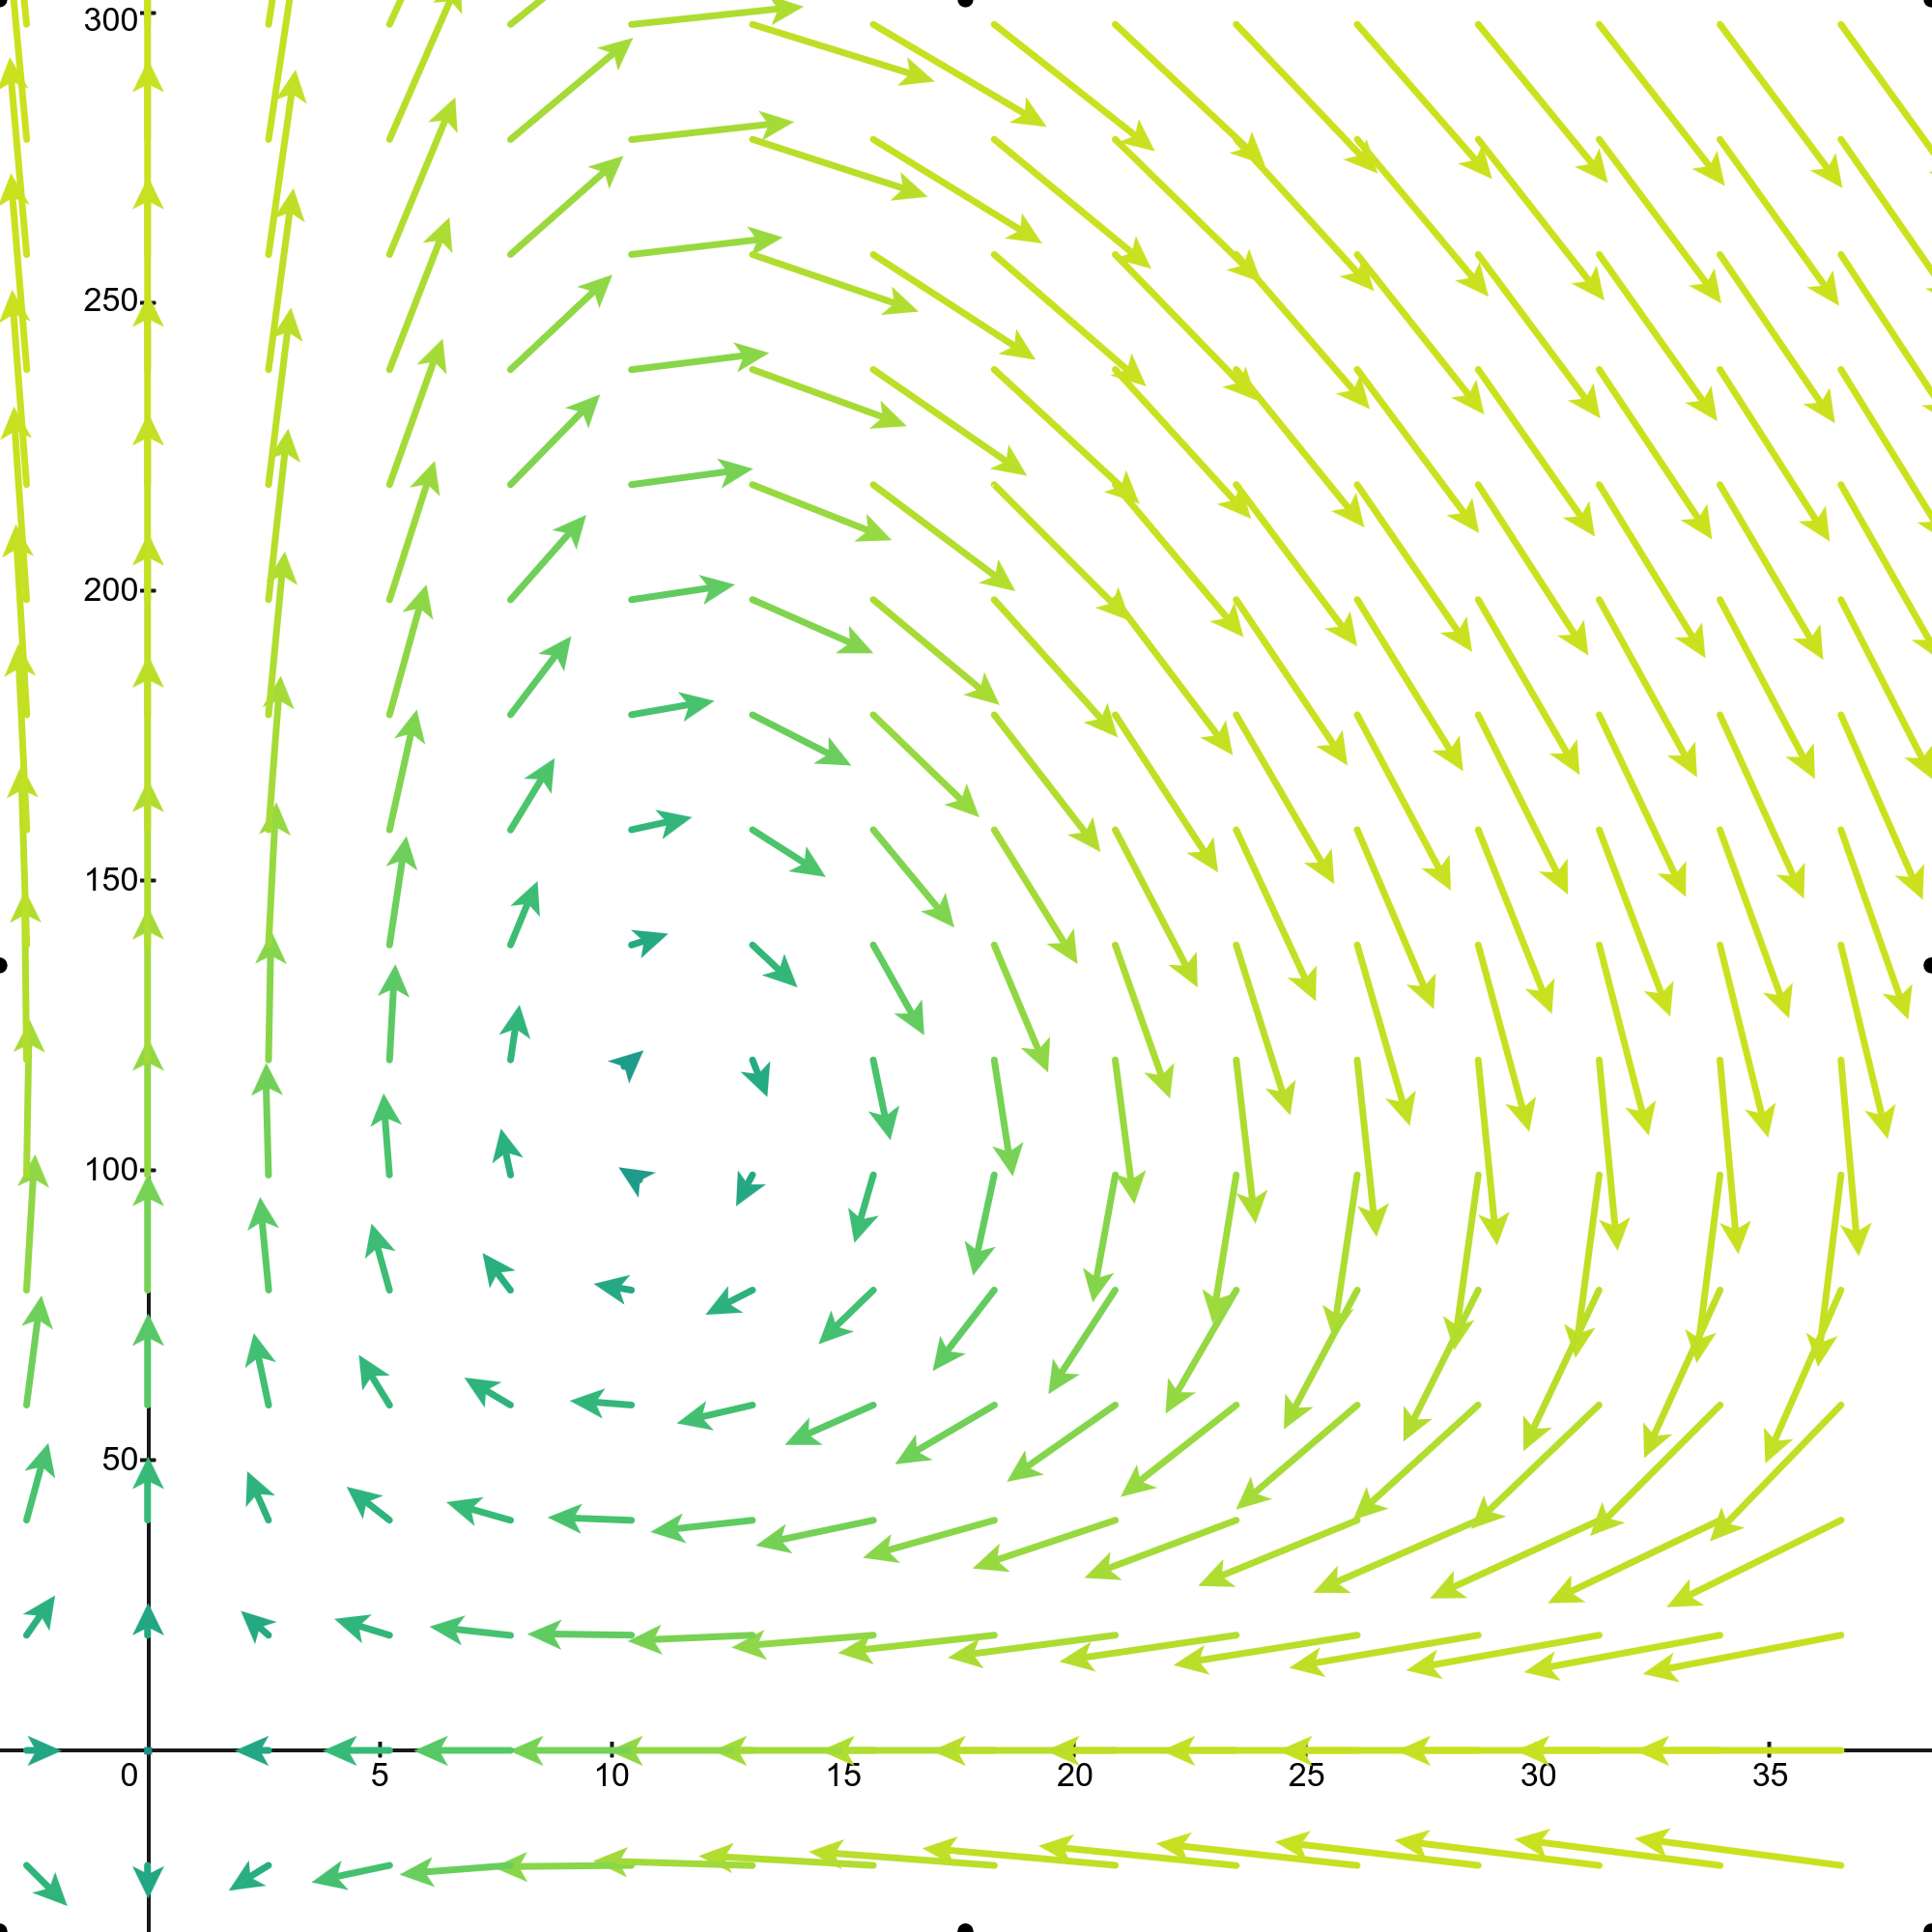
\includegraphics[width=3in]{resources/tutorial-02-1a.png}

				\item Arrows to the right of $F=11$ point down. That means as there are more foxes, the rabbit population decreases.
				Arrows to the left of $F=11$ point up, so as there are fewer foxes, there are more rabbits. If the arrows were oriented in the opposite direction,
				more foxes would lead to more rabbits, which is the opposite of what we would expect if the foxes ate the rabbits.
			\end{enumerate}
			\item \begin{enumerate}
				\item As long as $a,b,c,d>0$, there will be periodic behaviour.
				However, if any of the parameters becomes zero, the behaviour will change.
				\item 
				\item If we leave $a,c,d$ as they are and set $b$ to zero, the foxes will never die.
				Thus, the fox population will grow and grow as long as there are rabbits available. However,
				once the foxes eat the rabbits to extinction, they fox population will be unchanged, since the foxes are
				immortal!
			\end{enumerate}
			\item \begin{enumerate}
				\item We know that a maximum rabbit population occurs when $R'=0$. Manipulating the equation for
				$R'$, we find that $R'=0$ when $F=c/d$.
				\item Manipulating the equation for $F'$, we find that $F'=0$ when $R=b/a$.
				\item If neither populations change, then we must have $F'=0$ and $R'=0$. This occurs when
				$(F,R)=(c/d, b/a)$ or $(F,R)=(0,0)$.
				\item If we allow $d$ or $a$ to be zero, the derivations we did in the previous parts
				are no longer valid (we can't divide by zero)! If $c$ or $d$ equals zero, then there are equilibrium solutions
				where one population is positive and the other zero. Since populations cannot be negative, this prevents
				periodic behaviour. So, our analysis here helps explain part \ref{qual}.
			\end{enumerate}
		\end{enumerate}

	
	\end{solutions}
	\begin{instructions}
		\subsection*{Learning Objectives}
	Students need to be able to\ldots
	\begin{itemize}
		\item Switch between phase portraits and component graphs.
		\item Recognize the difference between solutions and curves in phase space.
		\item Deduce properties of equilibrium solutions from phase portraits.
	\end{itemize}

\subsection*{Context}
	We have analyzed systems of ODEs in class and in tutorial using phase portraits. We are getting ready to
	study systems of ODEs and equilibrium solutions to system written in matrix form. This requires a very good
	understanding of phase portraits and how they relate to solutions to systems.

\subsection*{What to Do}
	Introduce the learning objectives for the day's tutorial. Explain that phase portraits/graphs in phase space are an important
	tool in the study of differential equations and we want to better understand how graphs in phase space
	relate to solutions to systems of ODEs.

	Start by asking students to recall what we mean when we say ``phase portrait'' and ``component space'' for a system of ODEs
	$A'(t)=\ldots$ and $B'(t)=\ldots$. \emph{Do not give a lecture on this}, but you may have a short discussion ($< 5$ min)
	on this distinction.
	
	After most groups have finished \#1, go over it as a class. Doing so will ensure everyone has a baseline understanding
	of the distinction between phase space and component space.

	Continue as usual, walking around the room and asking
		questions while letting students work on the next problem and gathering them together
		for discussion when most groups have finished.

		7 minutes before class ends, pick a suitable problem to do as a wrap-up. Most likely, \#3 will be a good choice.



	
\subsection*{Notes}
	\begin{enumerate}
		\item Hopefully this problem won't be hard for them. All the vertices line up, after all. If they are struggling,
		it is worth spending a lot of time on this question, since they cannot use phase portraits unless they understand this.

		\item Students will struggle getting a curve for this question. If they are struggling, have them approximate
		the curve with a polygon and try to find component graphs for the polygon first. Then they can ``smooth it out''
		to get the curve.
		
		Part (b) will be especially hard. Some will struggle to even understand what the question is asking.

		\item This question is a good wrap-up question. It should be quicker than all the other questions.

		\item This is a question for groups who have moved more quickly. Students may have forgotten what an equilibrium
		solution is. Ask them to check their notes for the definition.

		Part (c) introduces a brand new definition. Assure students that they have not learned this definition in class
		and that's okay!

	\end{enumerate}
	\end{instructions}

\end{document}
